


\section{影像辨識}
處理的問題包含影像分類、物件偵測、實例分割

\subsection{ Convolution Neural Network (CNN)}

CNN 即捲積神經網路

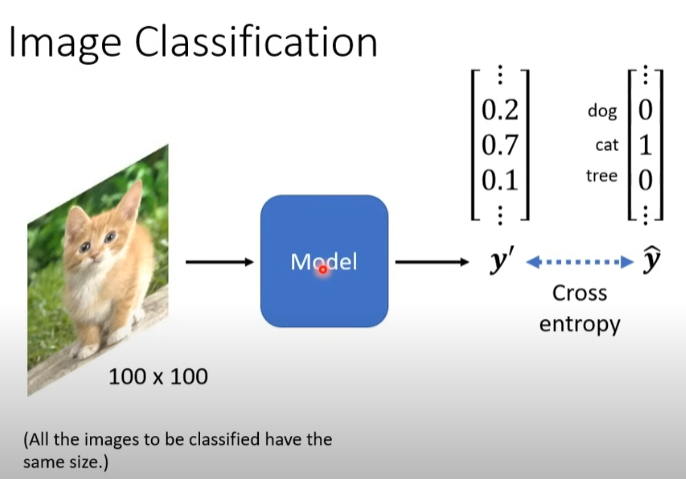
\includegraphics[width=.8\textwidth]{paste_src/2025-03-20-14-53-32.png}

以圖片分類任務為例子,輸入是 $100 \times 100 \ times 3 $ 的 Tensor,如果用 原本的全連接神經網路參數會非常多,model 的 彈性很大,也容易遇到 Overfitting。CNN 是一種降低彈性的神經網路。

\begin{align*}
  \mbox{Input} \rightarrow \mbox{Decoder} \rightarrow \mbox{Classifier} \rightarrow \mbox{Output}
\end{align*}

\subsection*{Decoder} 
Decoder 負責提取圖片特徵


\noindent\begin{minipage}[t]{.45\linewidth}\vspace{0pt}
  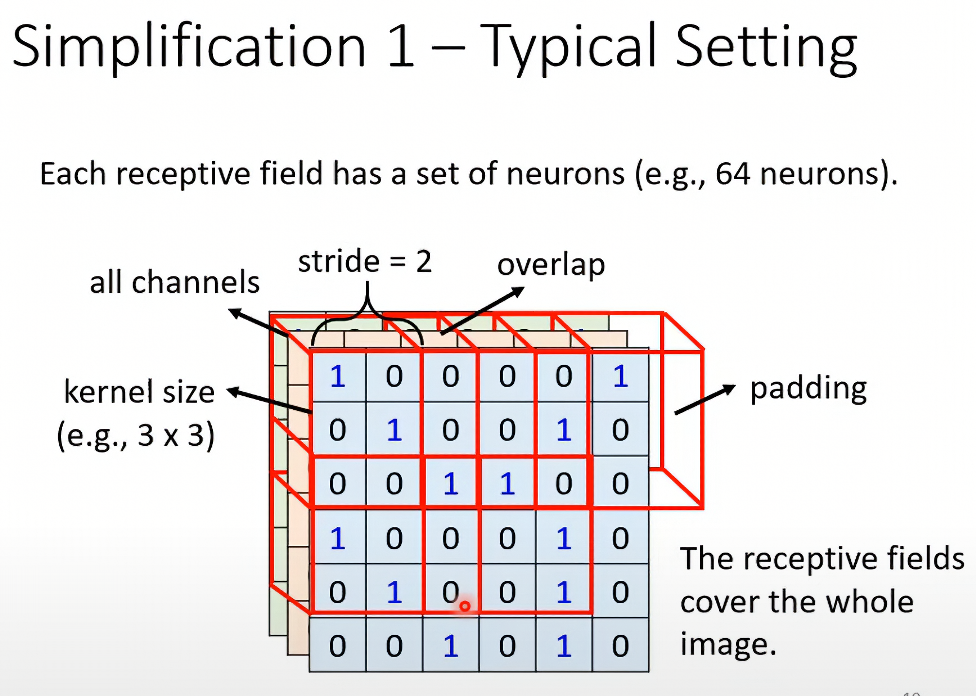
\includegraphics[width=1\textwidth]{paste_src/2025-03-20-15-08-14.png}
\end{minipage}
\begin{minipage}[t]{.45\linewidth}\vspace{0pt}
  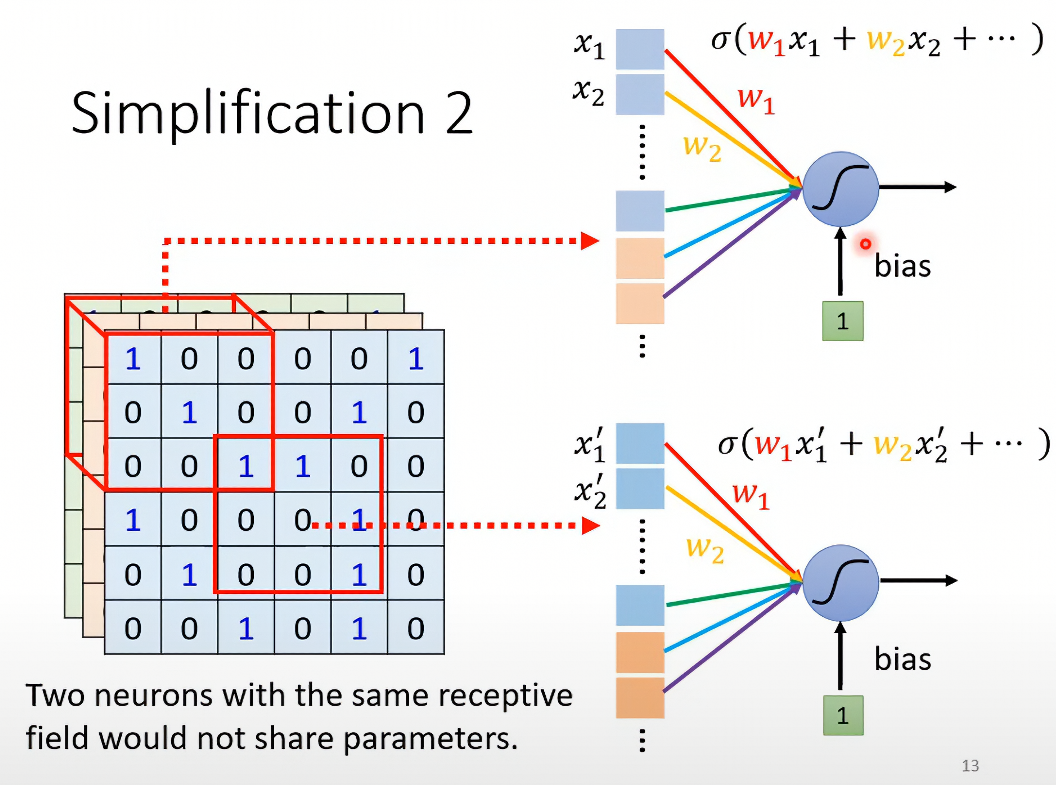
\includegraphics[width=1\textwidth]{paste_src/2025-03-20-15-13-31.png}
\end{minipage}


\section*{參考資料} 

\begin{enumerate}
  \item 【機器學習2021】機器學習任務攻略 -- 李宏毅
  \item 【機器學習2021】卷積神經網路 (Convolutional Neural Networks, CNN) ---- 李宏毅
\end{enumerate}
